\documentclass[a4paper]{scrartcl}

\usepackage[
typ=ib,
fach=Mathematik,
lerngruppe=2BF,
farbig,
namensfeldAnzeigen,
datumAnzeigen,
seitenzahlen = auto,
loesungen = seite,
module= {Papiertypen}
]{schule}


\usepackage{amsmath}
\usepackage{float}
\usepackage[]{fourier-otf}
\usepackage{microtype}	
\author{Maximilian Hertenstein}
\date{\today}
\title{Geraden-Punktprobe}
\date{Datum: \hspace{1.5cm}}

\usepackage{tkz-base}
\usepackage{tkz-fct}
\usepackage{tkz-euclide}
\ifoot{% TODO: \usepackage{graphicx} required

		
\includegraphics[width=0.3\linewidth]{GHSE-Logo}

}

\begin{document}




\begin{minipage}{0.5\linewidth}
\begin{center}
	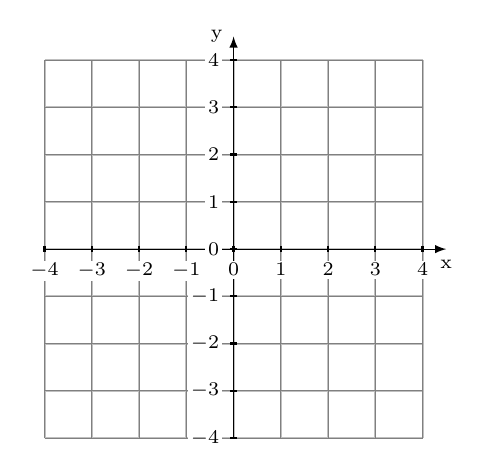
\begin{tikzpicture}[scale=.6]
		\scriptsize
		\tkzInit[ymax=4, xmax=4, xmin=-4, ymin=-4, xstep=1, ystep=1]
		\tkzGrid[sub,subxstep=1,subystep=1]
		\tkzFct[samples=50,domain=-5:5]{2*x-4}
		\tkzAxeXY[/tkzdrawX/label=x,/tkzdrawY/label=y]
	\end{tikzpicture}



$$f: y = $$

\end{center}
\end{minipage}
\begin{minipage}{0.5\linewidth}
\begin{center}
	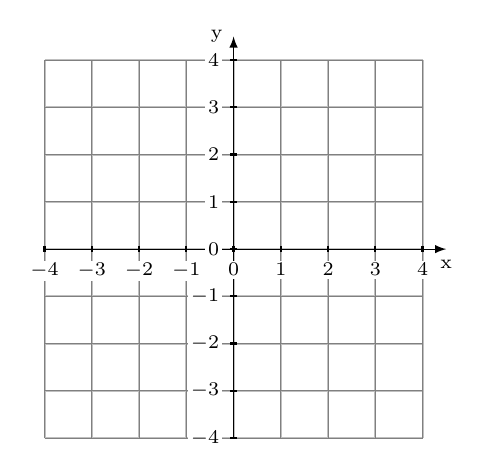
\begin{tikzpicture}[scale=.6]
		\scriptsize
		\tkzInit[ymax=4, xmax=4, xmin=-4, ymin=-4, xstep=1, ystep=1]
		\tkzGrid[sub,subxstep=1,subystep=1]
		\tkzFct[samples=50,domain=-5:5]{3-x}
		\tkzAxeXY[/tkzdrawX/label=x,/tkzdrawY/label=y]
	\end{tikzpicture}


$$g: y = $$

\end{center}
\end{minipage}


\section*{Schnittpunk mit y-Achse}
Um zu prüfen, ob ein Punkt, \begin{itemize}
\item auf
\item oberhalb
\item oder unterhalb
\end{itemize}

einer Geraden ist, setzt mann die $x$-Koordinate des Punkts für $x$ in die Geradengleichung ein.
Anschließend vergleicht man das berechnte $y$ mit der $y$-Koordinate des Punkts.

\textbf{Beispiel:}

\begin{minipage}{0.5\linewidth}
$$P(3 \mid 1)$$
\feldKar{13}
Der Punkt $P$ liegt \qquad\quad der Gerade $f$.
\end{minipage}
\begin{minipage}{0.5\linewidth}
$$P(1 \mid 2)$$
\feldKar{13}
Der Punkt $P$ liegt \qquad\quad der Gerade $g$.
\end{minipage}





\end{document} 